\begin{frame}
\frametitle{NAMD}
%
\begin{itemize}
\item
\end{itemize}
%
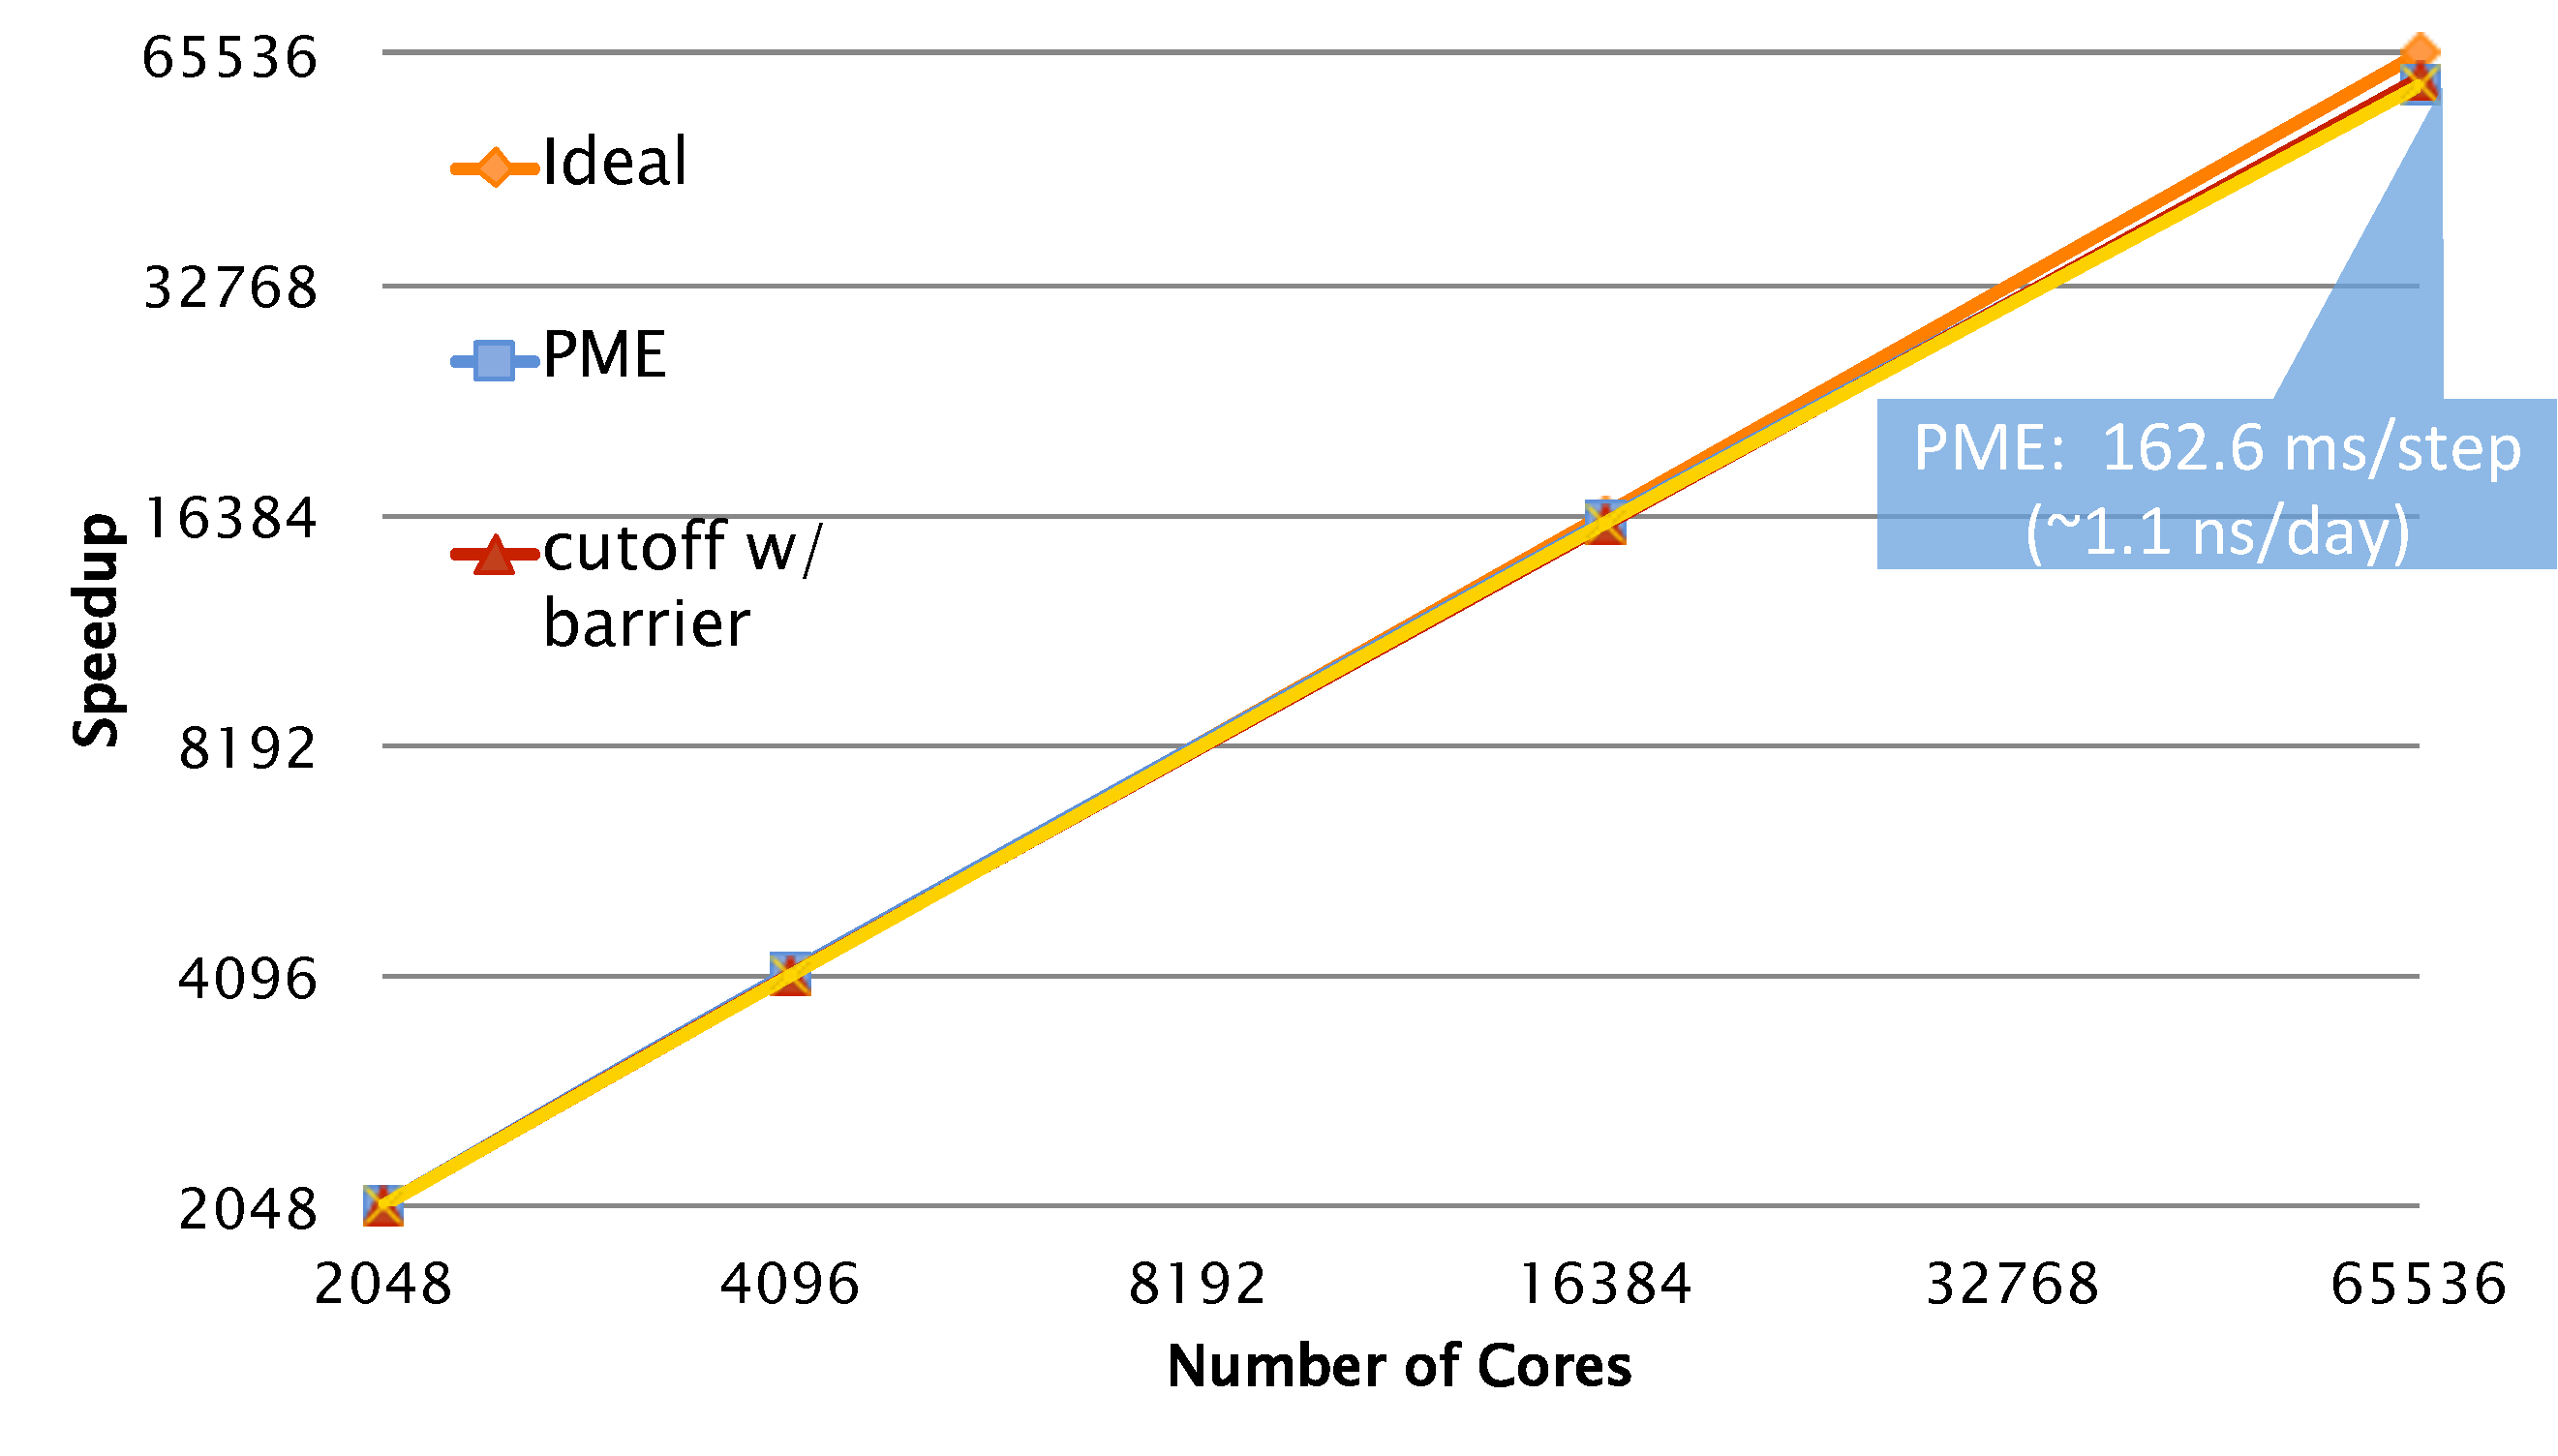
\includegraphics[width=0.5\textwidth]{../figures/namd_bgp.pdf}
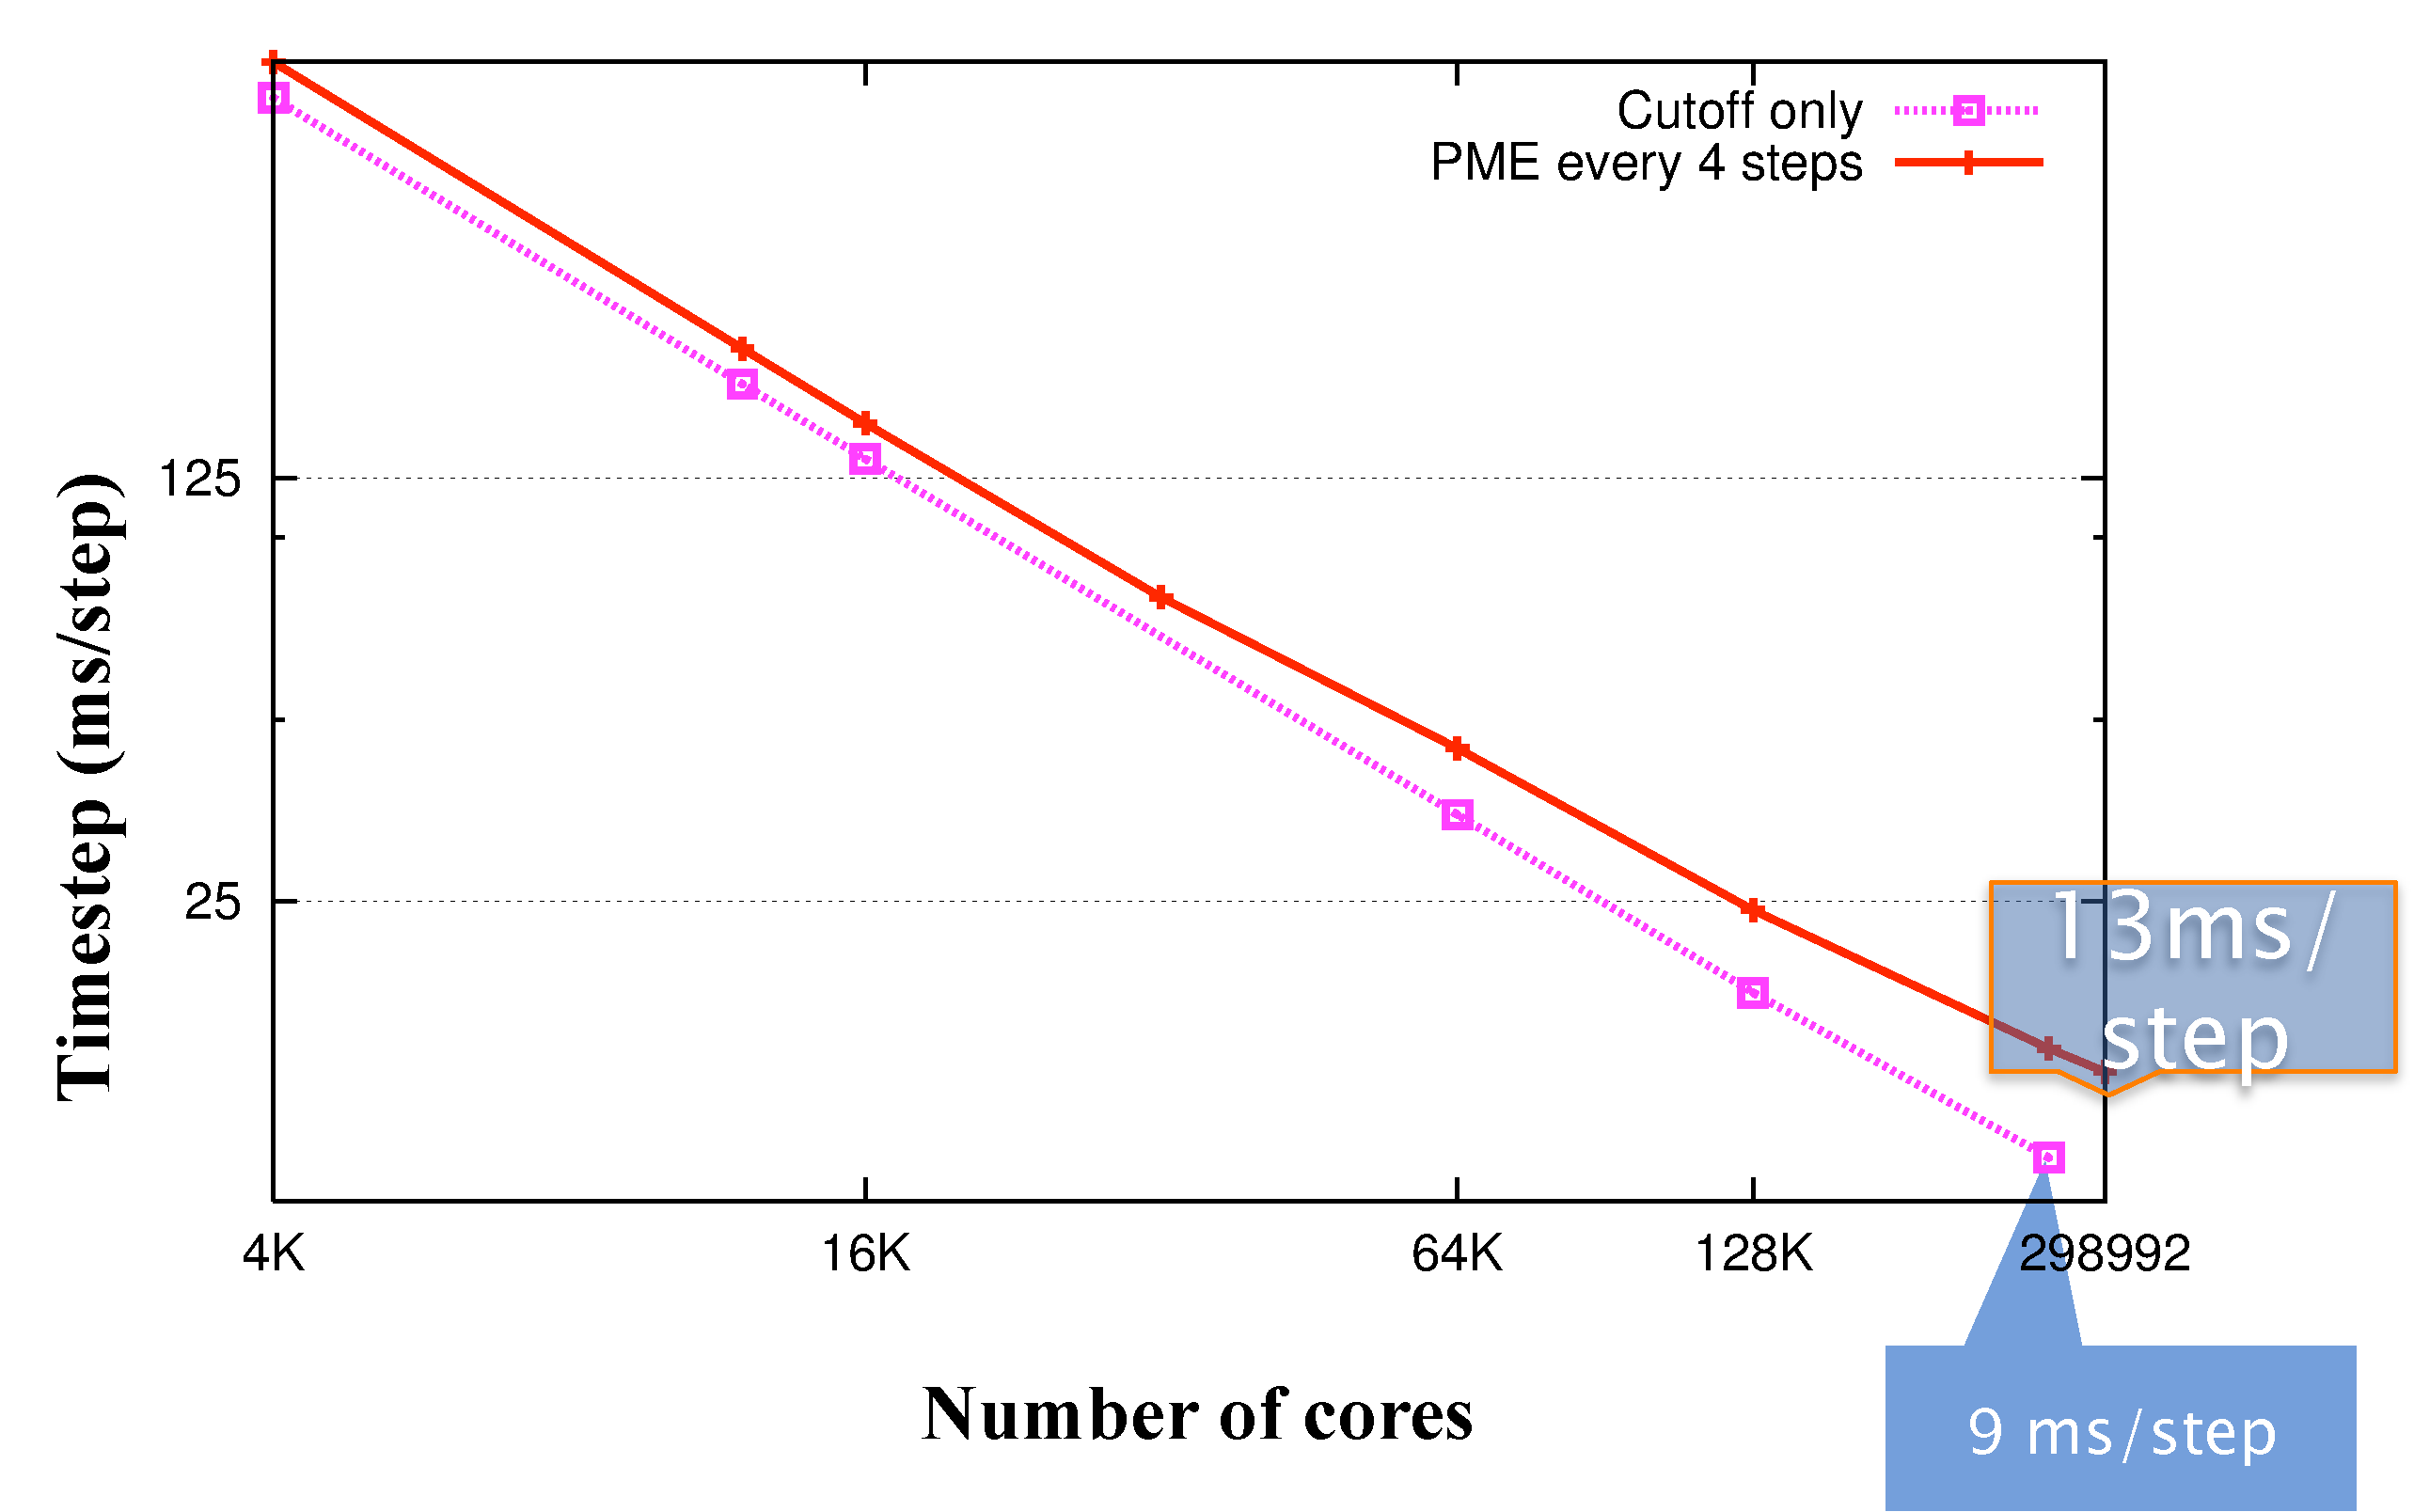
\includegraphics[width=0.5\textwidth]{../figures/namd_titan.pdf}
\end{frame}

\begin{frame}
\frametitle{ChaNGa}
%
\begin{itemize}
\item
\end{itemize}
%
%\includegraphics{../figures/}
\end{frame}

\begin{frame}
\frametitle{OpenAtom}
%
\begin{itemize}
\item
\end{itemize}
%
%\includegraphics{../figures/}
\end{frame}

\begin{frame}
\frametitle{Simdemics}
%
\begin{itemize}
\item
\end{itemize}
%
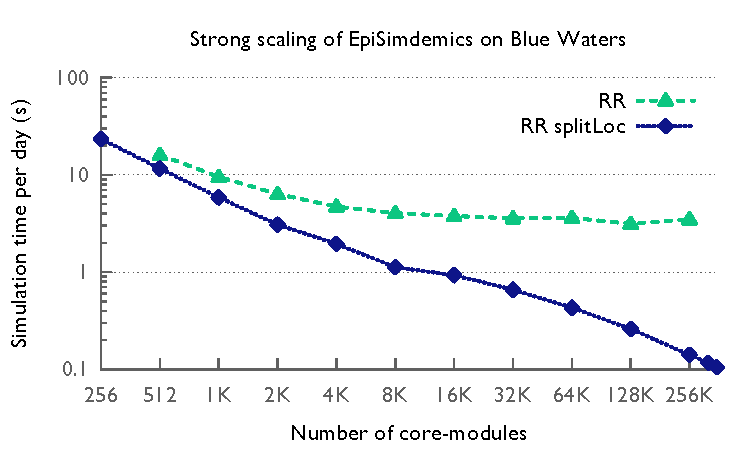
\includegraphics[scale=0.8]{../figures/simdemics_strong_scaling.pdf}
\end{frame}

\begin{frame}
\frametitle{JetAlloc}
%
\begin{itemize}
\item
\end{itemize}
%
%\includegraphics{../figures/}
\end{frame}

\begin{frame}
\frametitle{AMR}
%
\begin{itemize}
\item
\end{itemize}
%
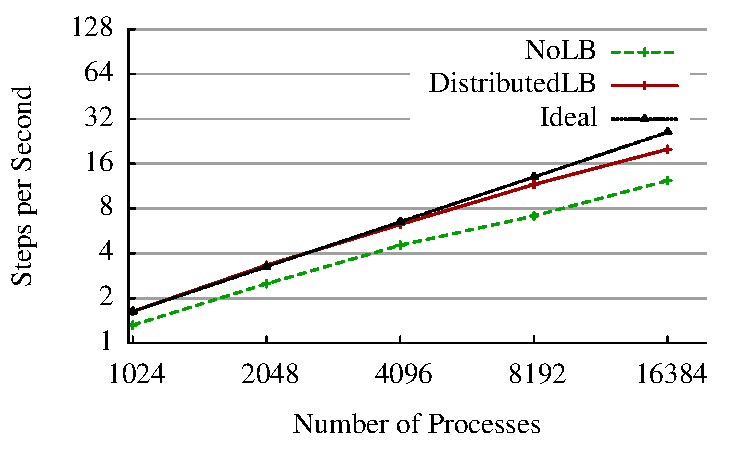
\includegraphics[scale=0.7]{../figures/amr_scaling_distlb.pdf}
\end{frame}

\begin{frame}
\frametitle{kdTree SMP}
%
\begin{itemize}
\item
\end{itemize}
%
%\includegraphics{../figures/}
\end{frame}

\begin{frame}
\frametitle{Numerical Linear Algebra}
%
Sparse Triangular Solver vs. SuperLU\_Dist
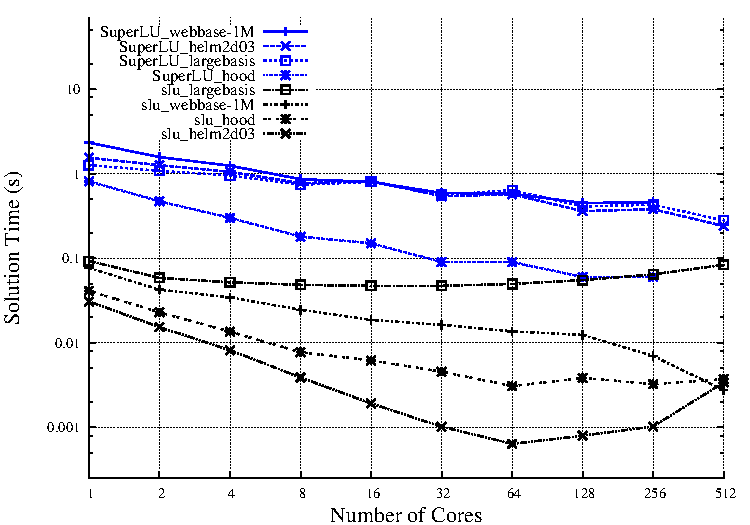
\includegraphics[scale=0.45]{../figures/sparselu_superlu_comparison.pdf}\\
Dense factorization: CharmLU
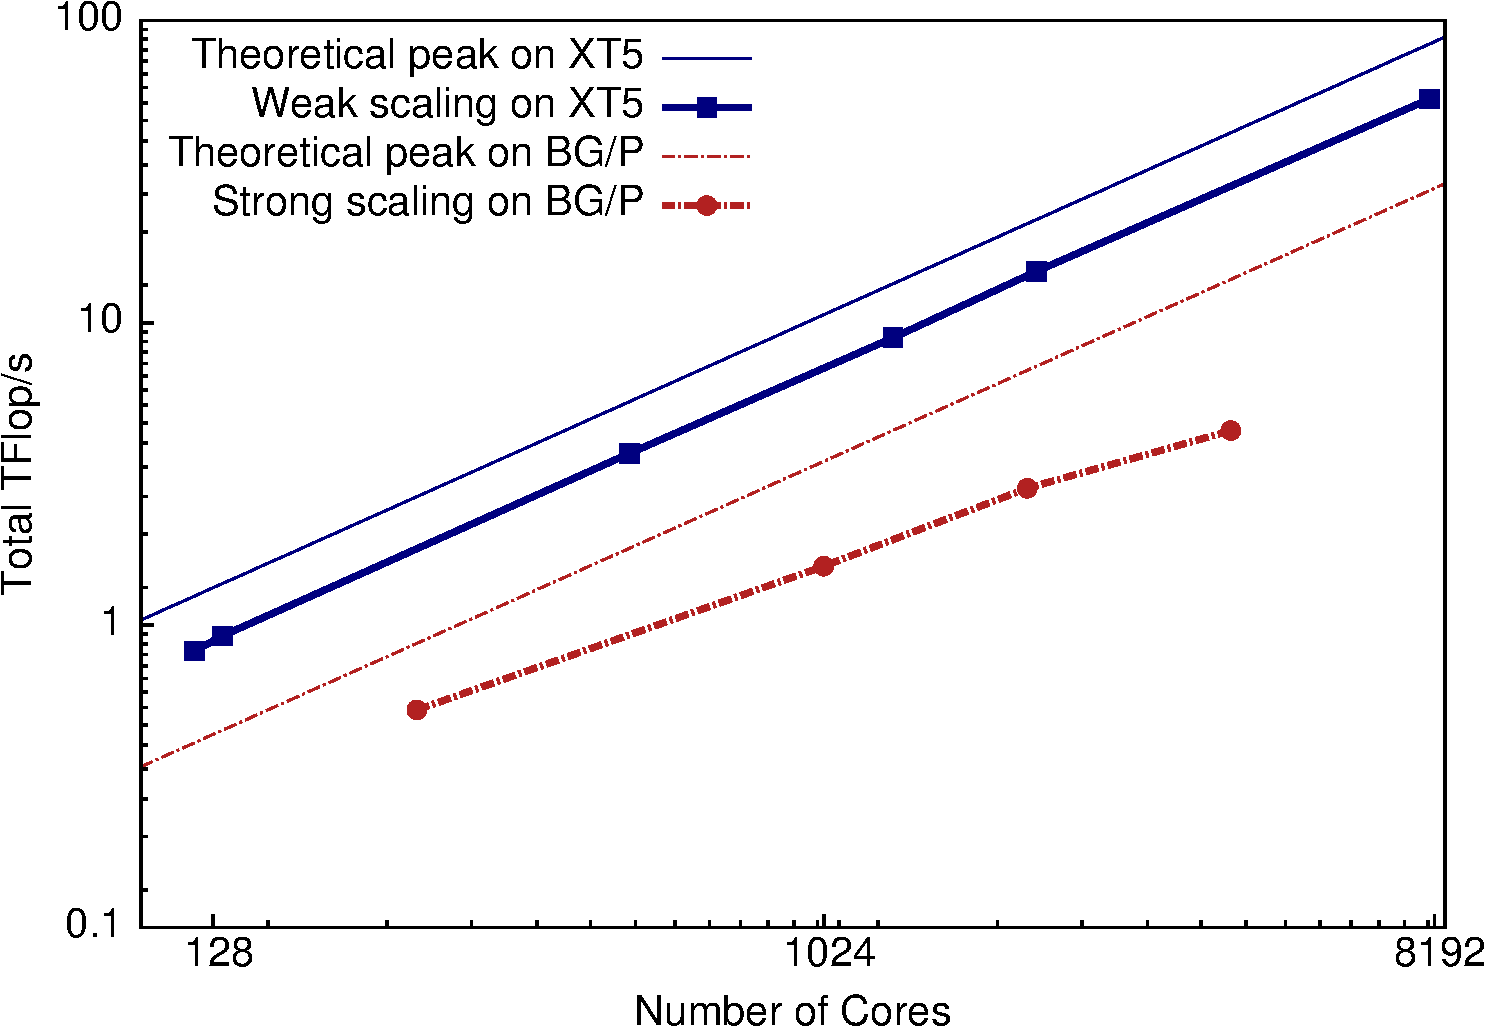
\includegraphics[scale=0.2]{../figures/charmlu_scaling.pdf}
\end{frame}

